In multi-target tracking, the posterior density cannot be described in a simple Gaussian distribution. Generally, the posterior distribution can have any form with only assumption that the integral of it sums to one. However, when we are dealing with Gaussian-linear cases, the posterior density is often represented as a mixture of many Gaussian components. A Gaussian mixture is a linear combination of multiple Gaussian distributions and its pdf is expressed in the following way:

\begin{equation}\label{eq:gaussian-mixture}
    p(\mathbf{x}) = \sum_{i=1}^N w_i \mathscr{N}\left(\mathbf{x}; \boldsymbol{\mu}_i, \Sigma_i\right),
\end{equation}

\noindent where $N$ is the number of Gaussian components in the mixture, $w_i$ is the weight of the $i$th component, the weights $w_i \geq 0$ sum to one, i.e. $\sum_{i=1}^N w_i = 1$, and each component $\mathscr{N}\left(\mathbf{x}; \boldsymbol{\mu}_i, \Sigma_i\right)$ is a Gaussian distribution with the mean in $\boldsymbol{\mu}_i$ and the covariance matrix $\Sigma_i$. An example of a Gaussian mixture pdf is illustrated in Figure \ref{fig:gaussian-mixture}.

\begin{figure}
\centering
  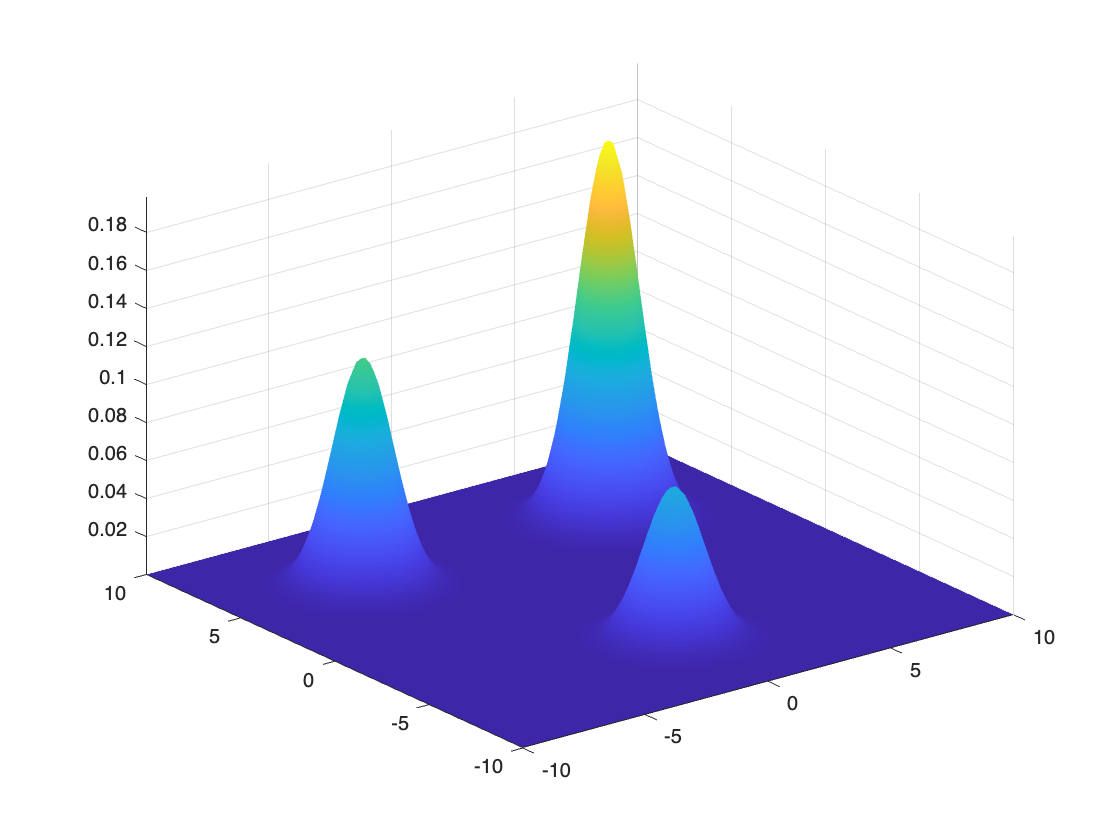
\includegraphics[width=.6\linewidth]{figures/gaussian-mixture.png}
  \caption[An example of a Gaussian mixture.]{An example of a Gaussian mixture with three components. The first component is centered at $[0, -5]^\intercal$ with weight $0.2$, the second component has mean in $[-5, 5]^\intercal$ with weight $0.3$ and the last has mean $[5, 5]^\intercal$ and the weight $0.5$.}
  \label{fig:gaussian-mixture}
\end{figure}

Since the weights sum to one, the Gaussian mixture satisfies the normalization requirement of pdfs and is thus a valid probability density function itself. The weights in the mixture represent the relative importance of the corresponding component. Gaussian mixtures are used to model complex distributions and have several nice mathematical properties as the Gaussian distribution, as we will later see. That is why Gaussian mixtures are widely used to represent posterior distributions in many MTT filters. Moreover, one can easily approximate any distribution with a Gaussian mixture using algorithms such as the Expectation-Maximization algorithm \cite{hastieElementsStatisticalLearning2001}.

A mixture $f(\mathbf{X})$ with $N$ components will have the expected value $\boldsymbol{\hat{\mu}}$ and the covariance $\hat{\Sigma}$ according to the following equations:

\begin{align}
    \boldsymbol{\hat{\mu}} &= \sum_{i=1}^N w_i \boldsymbol{\mu}_i, \\
    \hat{\Sigma} &= \sum_{i=1}^N w_i \Sigma_i + \Tilde{\Sigma},
\end{align}

\noindent where the term $\Tilde{\Sigma}$ is called the spread-of-the-innovations and is defined as:

\begin{equation}
    \Tilde{\Sigma}= \sum_{i=1}^N
        w_i (\boldsymbol{\mu}_i - \hat{\boldsymbol{\mu}})
        (\boldsymbol{\mu}_i - \hat{\boldsymbol{\mu}})^\intercal.
\end{equation}

The spread-of-the-innovations quantifies the magnitude of the difference between expectations of individual components.
